% ============================================================
%  Figure 9 — Short-window fit quality (L = 80 ms)
% ============================================================
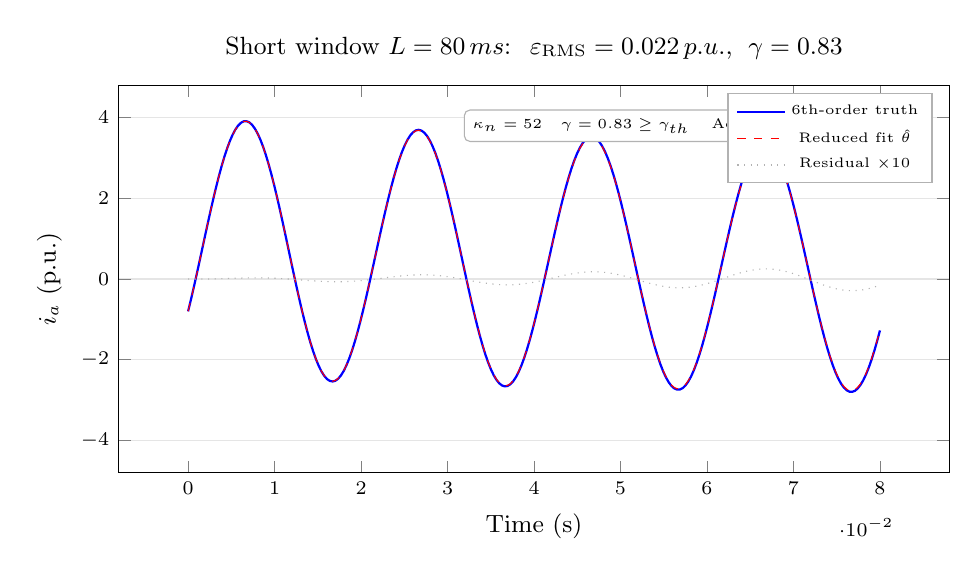
\begin{tikzpicture}
\begin{axis}[
  width=\columnwidth, height=6.5cm,
  domain=0:0.08, samples=250,
  xlabel={Time (s)},
  ylabel={$i_a$ (p.u.)},
  ymin=-4.8, ymax=4.8,
  ymajorgrids=true, grid style={gray!20},
  label style={font=\small},
  tick label style={font=\scriptsize},
  title={Short window $L = 80\,\text{ms}$:\;
         $\varepsilon_{\mathrm{RMS}} = 0.022\,\text{p.u.}$,\;
         $\gamma = 0.83$},
  title style={font=\small},
  legend style={at={(0.98,0.98)}, anchor=north east,
                font=\tiny, fill=white, draw=black!30},
  clip=false
]

% 6th-order truth
\addplot[blue, thick, solid] {
  (1.35*(1+0.15*(1-exp(-x/0.5))) + 1.85*exp(-x/0.83))
  * sin(deg(314.16*x) - 30)
  + 1.60*0.5*exp(-x/0.07)
};

% Reduced fit (near-identical over 80ms window)
\addplot[red, dashed] {
  (1.35 + 1.85*exp(-x/0.83)) * sin(deg(314.16*x) - 30)
  + 1.60*0.5*exp(-x/0.07)
};

% Residual x10
\addplot[gray!60, dotted] {
  10 * 1.35*0.15*(1-exp(-x/0.5))*sin(deg(314.16*x) - 30)
};

\legend{6th-order truth, Reduced fit $\hat{\bm\theta}$, Residual $\times 10$};

% Annotation box
\node[draw=black!30, fill=white, rounded corners=2pt,
      font=\tiny, align=left, inner sep=3pt]
  at (axis cs:0.050, 3.8)
  {$\kappa_n = 52$\quad $\gamma = 0.83 \geq \gamma_{th}$\quad $\checkmark$\,Accept};

\end{axis}
\end{tikzpicture}
